
% =========================================================
\section{Introduction}
\begin{frame}
	\frametitle{Introduction}
	\framesubtitle{Business Understanding - Legislative Proposal's Definition and Types}

	\begin{exampleblock}{Legislative Proposal} 
	\begin{itemize}
		\item A \textbf{Legislative Proposal} is any matter subject to deliberation by the Legislative Chamber (CLDF Internal Regulations, art. 129).
	\end{itemize}
	\end{exampleblock}

	\begin{exampleblock}{} 
	\textbf{Legislative Proposals can be of the following types:}
	\begin{multicols}{2}
		\begin{itemize}
			\item Proposta de emenda à Lei Orgânica;
			
			\item Projeto de lei complementar;
			
			\item Projeto de lei;
			
			\item Projeto de decreto legislativo;
			
			\item Projeto de resolução;
			
			\item Indicação;
			
			\item Moção;
			
			\item Requerimento;
			
			\item Emenda;
			
			\item Recursos;
		\end{itemize}
	\end{multicols}
	\end{exampleblock}
\end{frame}
% --------------------------------------------------------------------------------------------
\begin{frame}
	\frametitle{Introduction}
	\framesubtitle{Business Understanding - Legislative Proposal's Themes}

	%https://ple.cl.df.gov.br/#/proposicao/buscar	
	\begin{exampleblock}{Legislative Proposals are classified into one or more themes:} 
		\begin{multicols}{3}
			\begin{itemize}
				\scriptsize
				\item Agricultura
				\item Assistência Social
				\item Assunto Fundiário e Ordenamento Territorial
				\item Assunto Social
				\item Cidadania
				\item Ciência e Tecnologia
				\item Combate à Corrupção
				\item Comunicação
				\item Comércio e Serviços
				\item Cultura
				\item Defesa do Consumidor
				\item Desenvolvimento Econômico
				\item Desporto e Lazer
				\item Direitos Humanos
				\item Economia
				\item Educação
				\item Energia
				\item Fiscalização e Governança
				\item Habitação
				\item Incentivos Fiscais e Concessões Públicas
				\item Indústria
				\item Meio Ambiente
				\item Não se aplica
				\item Outro
				\item Previdência Social
				\item Relações Exteriores
				\item Saneamento
				\item Saúde
				\item Segurança
				\item Servidor Público
				\item Trabalho
				\item Transporte e Mobilidade Urbana
				\item Turismo
				\item Urbanismo
				\normalsize
			\end{itemize}
		\end{multicols}
		\textbf{Total:} 34 themes	
	\end{exampleblock}
\end{frame}
% --------------------------------------------------------------------------------------------
\begin{frame}
	\frametitle{Introduction}
	\framesubtitle{Business Understanding - Why Themes?}
	\begin{block}{Thematic Classification Benefits} % Block without title
		\begin{itemize}
			\item Efficient classification of legislative proposals is crucial to \textbf{streamline their analysis} and processing within the legislative process helping to \textbf{determine which committees a proposal should go through}.
					
			% Otimizar a análise e o processamento dentro do processo legislativo, ajudando a determinar quais comissões uma proposta deve percorrer
					
			\item Thematic classification plays an important role in maintaining \textbf{accurate information retrieval} and \textbf{ensuring effective legislative management}.
			
			% Desempenha um papel importante na manutenção da recuperação precisa de informações e na garantia de uma gestão legislativa eficaz
			
			\item By categorizing legislative proposals into relevant themes, lawmakers can streamline their analysis, \textbf{allocate resources efficiently}, and \textbf{make informed decisions}. 
			
			% Alocar recursos de forma eficiente e tomar decisões informadas
				
			\item This process \textbf{enhances transparency} and facilitates a more \textbf{organized legislative workflow}.	
			% Melhora a transparência e facilita um fluxo legislativo mais organizado.
		\end{itemize}
	\end{block}
\end{frame}
% =========================================================
\section{The Problem}
\begin{frame}
	\frametitle{The Problem}
	\framesubtitle{Understanding the problem}
	\begin{alertblock}{Theme ``others'' is growing bigger}
		\begin{itemize}
			\item 	Usually, the author of the proposal is responsible for classifying it into one or more themes.
			
			% A escolha dos temas para classificação é feita pelo autor da proposição
			
			\item Unfortunately, due to various factors such as ambiguous topics, outdated categories, multidisciplinary nature, \textbf{many propositions end up being classified under the generic label of ``others''}.
			
			% Infelizmente, devido a diversos fatores, como tópicos ambíguos, categorias desatualizadas e natureza multidisciplinar, muitas proposições acabam sendo classificadas sob o rótulo genérico de “outros”.
			
		\end{itemize}
	\end{alertblock}	
\end{frame}
% --------------------------------------------------------------------------------------------
\begin{frame}
	\frametitle{The Problem}
	\framesubtitle{Understanding the problem}	
	\begin{figure}
		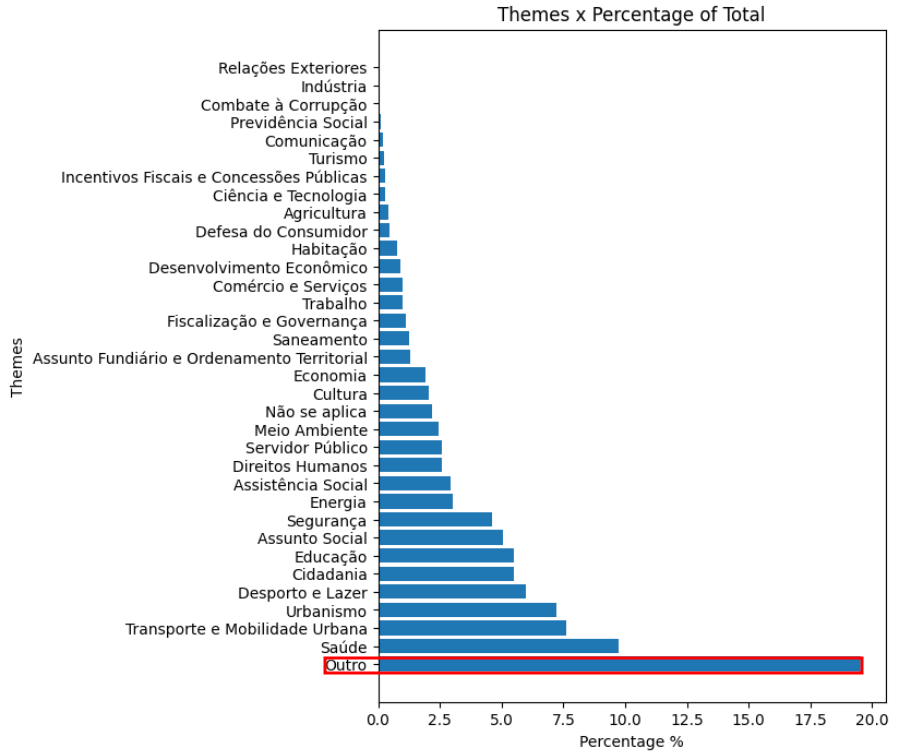
\includegraphics[width=0.6\linewidth]{graphThemes.png}
	\end{figure}

	\begin{block}{}
		\scriptsize
		The chart shows that the number of proposals classified under the theme “others” represents approximately 20\% of the total. 
	\end{block}	
\end{frame}
% --------------------------------------------------------------------------------------------
\begin{frame}
	\frametitle{The Problem}
	\framesubtitle{Problem definition}	

	\begin{alertblock}{The problem is inadequate proposal classification}
		Inadequate classification hinders efficient tracking, analysis, and transparency of legislative activities, making it difficult for both society and lawmakers to understand and oversee the legislative process effectively.
	\end{alertblock}	

	\begin{figure}
		
\includegraphics[width=0.3\linewidth]{problem.jpeg}
	\end{figure}


	% Essa classificação inadequada dificulta o acompanhamento eficiente, a análise e a transparência das atividades legislativas, tornando desafiador tanto para a sociedade quanto para os legisladores compreender e supervisionar efetivamente o processo legislativo. 
	
	

\end{frame}
% =========================================================
\section{Objective}
\begin{frame}
	\frametitle{Objective}
	
	\begin{block}{Objective} 
	\begin{itemize}
		\item The main goal is to create a model capable of sugesting new categorys for proposals classified under generic label ``others'' with themes that better suits that proposal.
	\end{itemize}
	\end{block}
		
	\begin{figure}
		
\includegraphics[width=0.3\linewidth]{arrow.jpeg}
	\end{figure}
		
	% O objetivo principal é criar um modelo capaz de sugerir novas categorias para propostas classificadas sob rótulo genérico ''outros'' com um ou mais temas que melhor se adaptem àquela proposta.
	
\end{frame}
% =========================================================
\section{Literature review}
\begin{frame}
	\frametitle{Literature review}
	
	Citar um ou dois artigos mais importantes.
	
	
\end{frame}
% =========================================================
\section{Methodology}
\begin{frame}
	\frametitle{Methodology}
	\begin{block}{CRISP-DM's Methodology} % Block without title
		\begin{enumerate}
			\item \textbf{Business Understanding}: We have analyzed legislative documents to align our data mining objectives with legislative classification needs.
			
			\item \textbf{Data Understanding}: The dataset comprises 22,267 summaries extracted from the Electronic Legislative Process (PLE) system, each accompanied by its respective thematic classification.
			
			\item \textbf{Data Preparation}: First, we discarded data classified under the 'Other' theme. Then, we performed tokenization, normalization, stopword removal, and lemmatization processes.
			
			\item (next slide)
		\end{enumerate}
	\end{block}
\end{frame}
% --------------------------------------------------------------------------------------------
\begin{frame}
	\frametitle{Methodology}
	\begin{block}{CRISP-DM's Methodology (cont...)} % Block without title
		\begin{enumerate}
			\setcounter{enumi}{3}
		
			\item \textbf{Modeling}: We use a multilingual sentence embedding model based on the MiniLM architecture, a lightweight and efficient BERT variant with 12 transformer layers, to produce high-quality embeddings for NLP tasks like semantic similarity, paraphrase identification and clustering.
			
			\item \textbf{Evaluation}: Our evaluation metrics include:
			\begin{enumerate}
				\item \textbf{Semantic Textual Similarity}: Pearson/Spearman correlation.
				
				\item \textbf{Paraphrase Identification}: Accuracy, F1 score, Precision, Recall.
				
				\item \textbf{Clustering}: Silhouette score, ARI, NMI.
			\end{enumerate}
	
			
			\item \textbf{Deployment}: The results will be used to create an interface in the PLE system to suggest themes that best fit new proposals.			
		\end{enumerate}
	\end{block}
\end{frame}
% =========================================================
\section{Experimentos Realizados}
\begin{frame}
	\frametitle{Experimentos Realizados}
	
	Falar do Embed
	
	
	
\end{frame}
% =========================================================
\section{Resultados}
\begin{frame}
	\frametitle{Resultados}
	
	
	
	
\end{frame}
% =========================================================
\section{Trabalhos Futuros}
\begin{frame}
	\frametitle{Resultados}
	
	
	
	
\end{frame}
% =========================================================
\section{Conclusões}
\begin{frame}
	\frametitle{Conclusões}
	
	
	
	
\end{frame}
% =========================================================




















